%%
%% 第一章 渲染情势
%% 2014.6.25
%% 	http://www.processon.com/#画流程图的软件

\chapter{绪论}
本章主要介绍基于局部特征的图像重建系统在基于云的图像压缩方面的应用场景,该技术的研究背景、国内外的发展情况以及目前取得的研究成果,最后介绍了本文的主要研究内容和文章的组织结构。


\section{论文课题的研究背景}

随着数字化时代的不断发展,智能终端日益普及,终端应用的功能也日趋多样化,我们发现有一类应用服务规模迅速扩大,这一类型的应用采用相似的CS技术架构——智能终端使用传感器采集图像数据,并通过网络向服务器实时传输,由服务器来处理数据,将处理结果反馈给终端用户。而图像应用的爆发式增长给我们带来了一个全新的挑战:图像信息的传输占用了大量的带宽资源。目前的解决方案是在终端对原始图像进行下采样和压缩编码,产生的图像信息的损失大大降低了用户体验,而且传统的压缩编码算法占用了一定的CPU资源,压缩比不是很高,压缩后的图像数据量依然较大。

另一方面,走在大数据时代前沿的互联网拥有无比丰富的图像资源,图像张数数以亿计,图像样式种类五花八门,而且每天还不断有用户贡献着高质量高分辨率的图像。从信息的角度来说,我们拍摄的每一幅图像中所包含的部分或全部内容都可以在互联网上其它图像中找到。

以上两点观察启示我们打破传统的图像内逐像素压缩方法,采用一种全新的基于大数据集的外部图像压缩方法。在2013年6月有学者\cite{Yue:2013gl}提出一种全新的压缩方式——基于云的图像编码。其核心思想是在客户端提取并编码发送少量的图像特征数据,并不传输图像数据本身,而在服务器端解码后利用特征数据在服务器的大图像数据集上匹配相似的图像,利用相似图像进行图像的重建。图\ref{fig:overview}展示了这一客户端-服务器(Client-Service)数据应用模式。这种架构所运用的核心技术手段便是基于局部特征的图像重建算法,通过对原始图像的特征提取与重建,利用计算资源减少带宽损耗,从一个全新的维度进行数据压缩,为多媒体应用开启了一扇大门。

\begin{figure}
\centering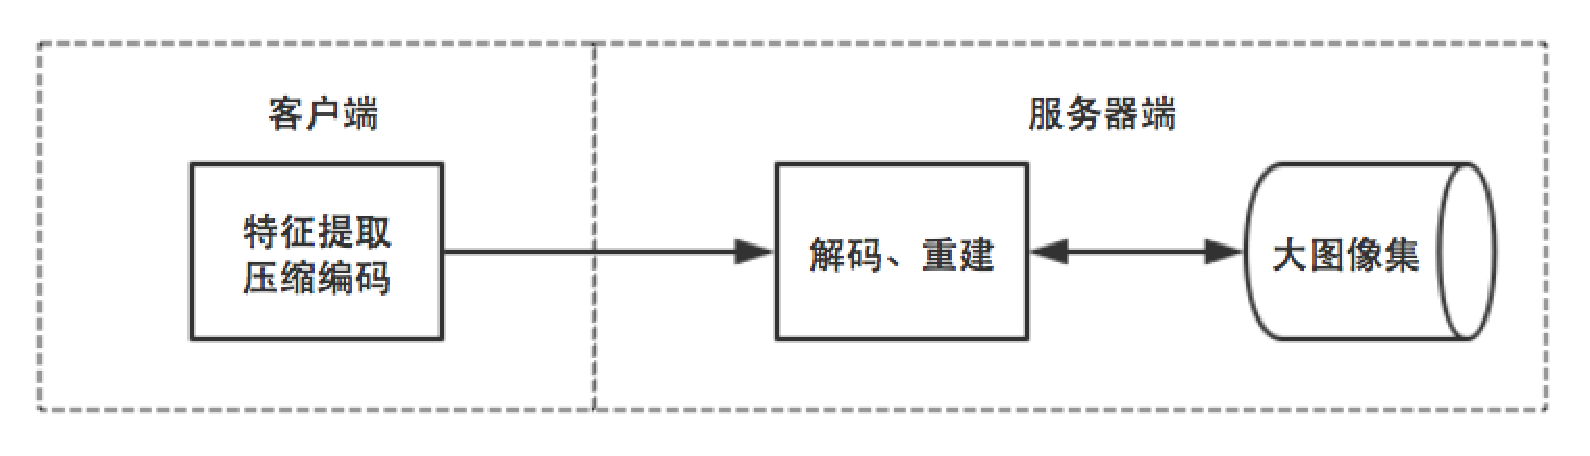
\includegraphics[width=14cm]{imgs/ch1/overview}
\caption{基于与的图像压缩模式}
\label{fig:overview}
\end{figure}

\begin{figure}
\centering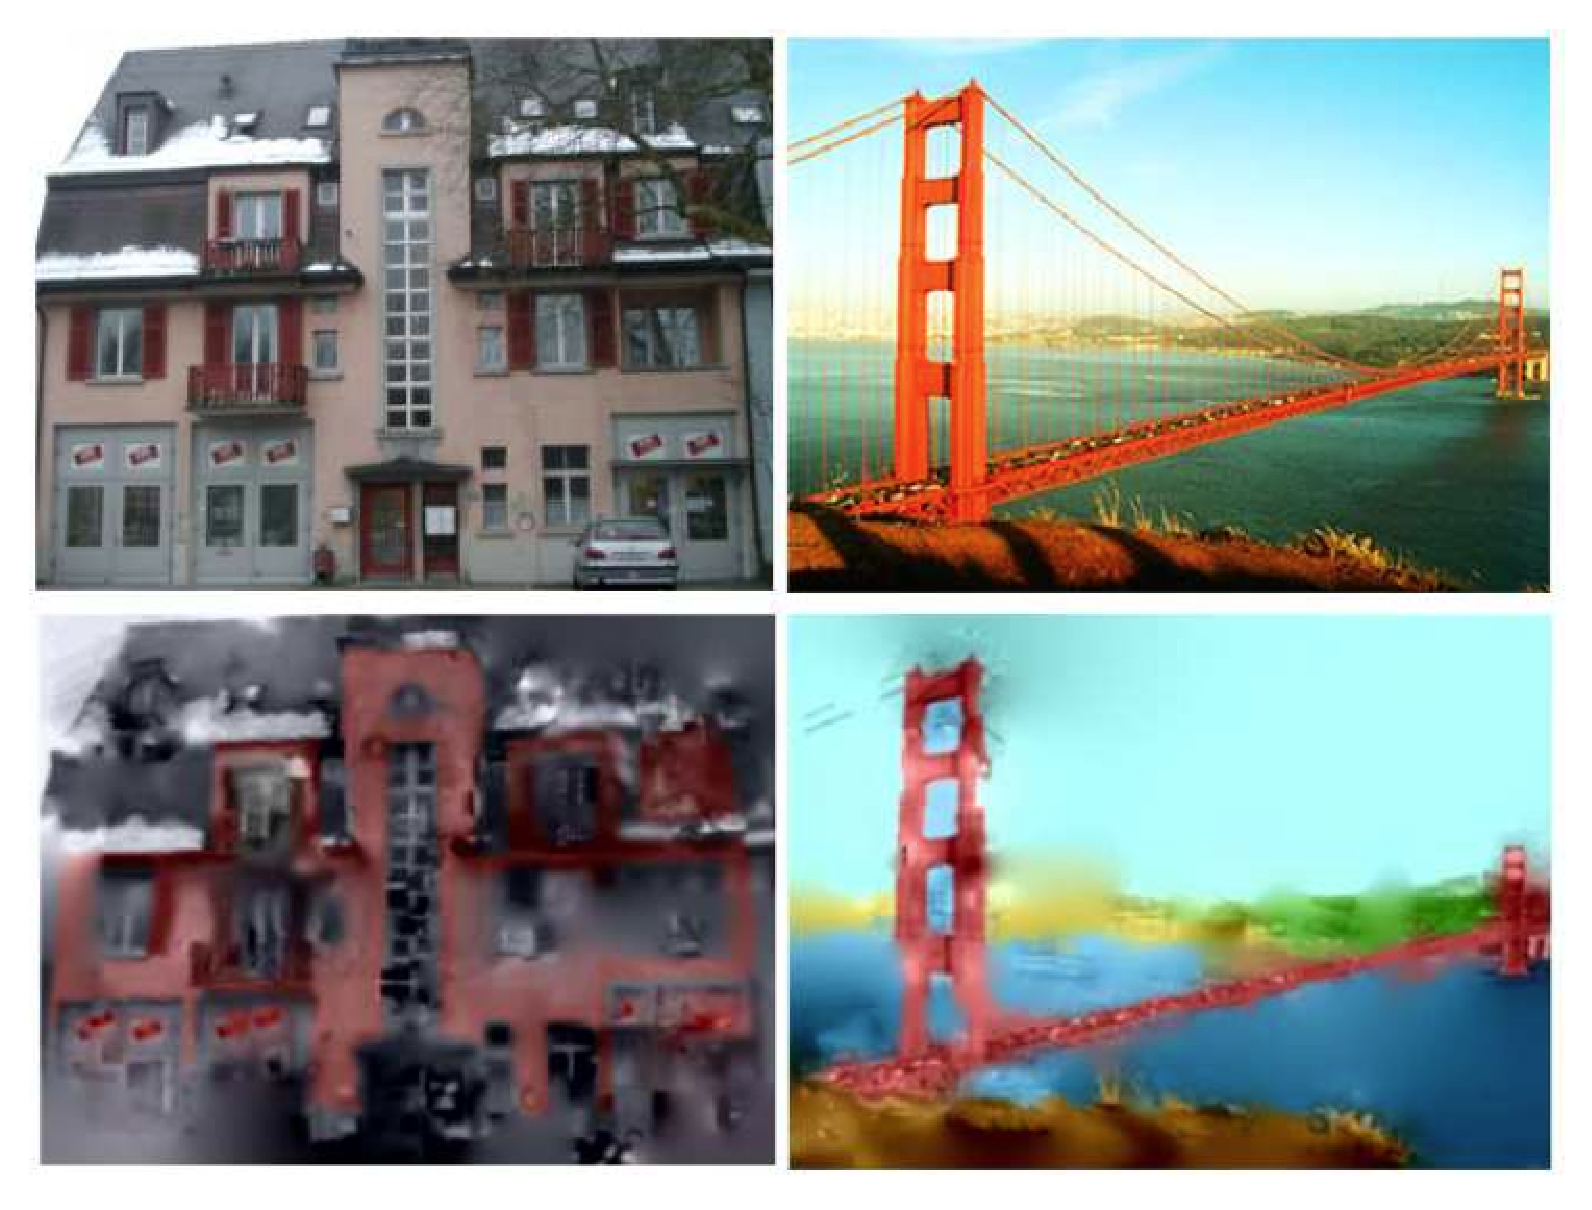
\includegraphics[width=12cm]{imgs/ch1/Daneshi_res}
\caption{Daneshi基于局部特征的图像重建结果}
\label{fig:Daneshi_res}
\end{figure}

\begin{figure}
\centering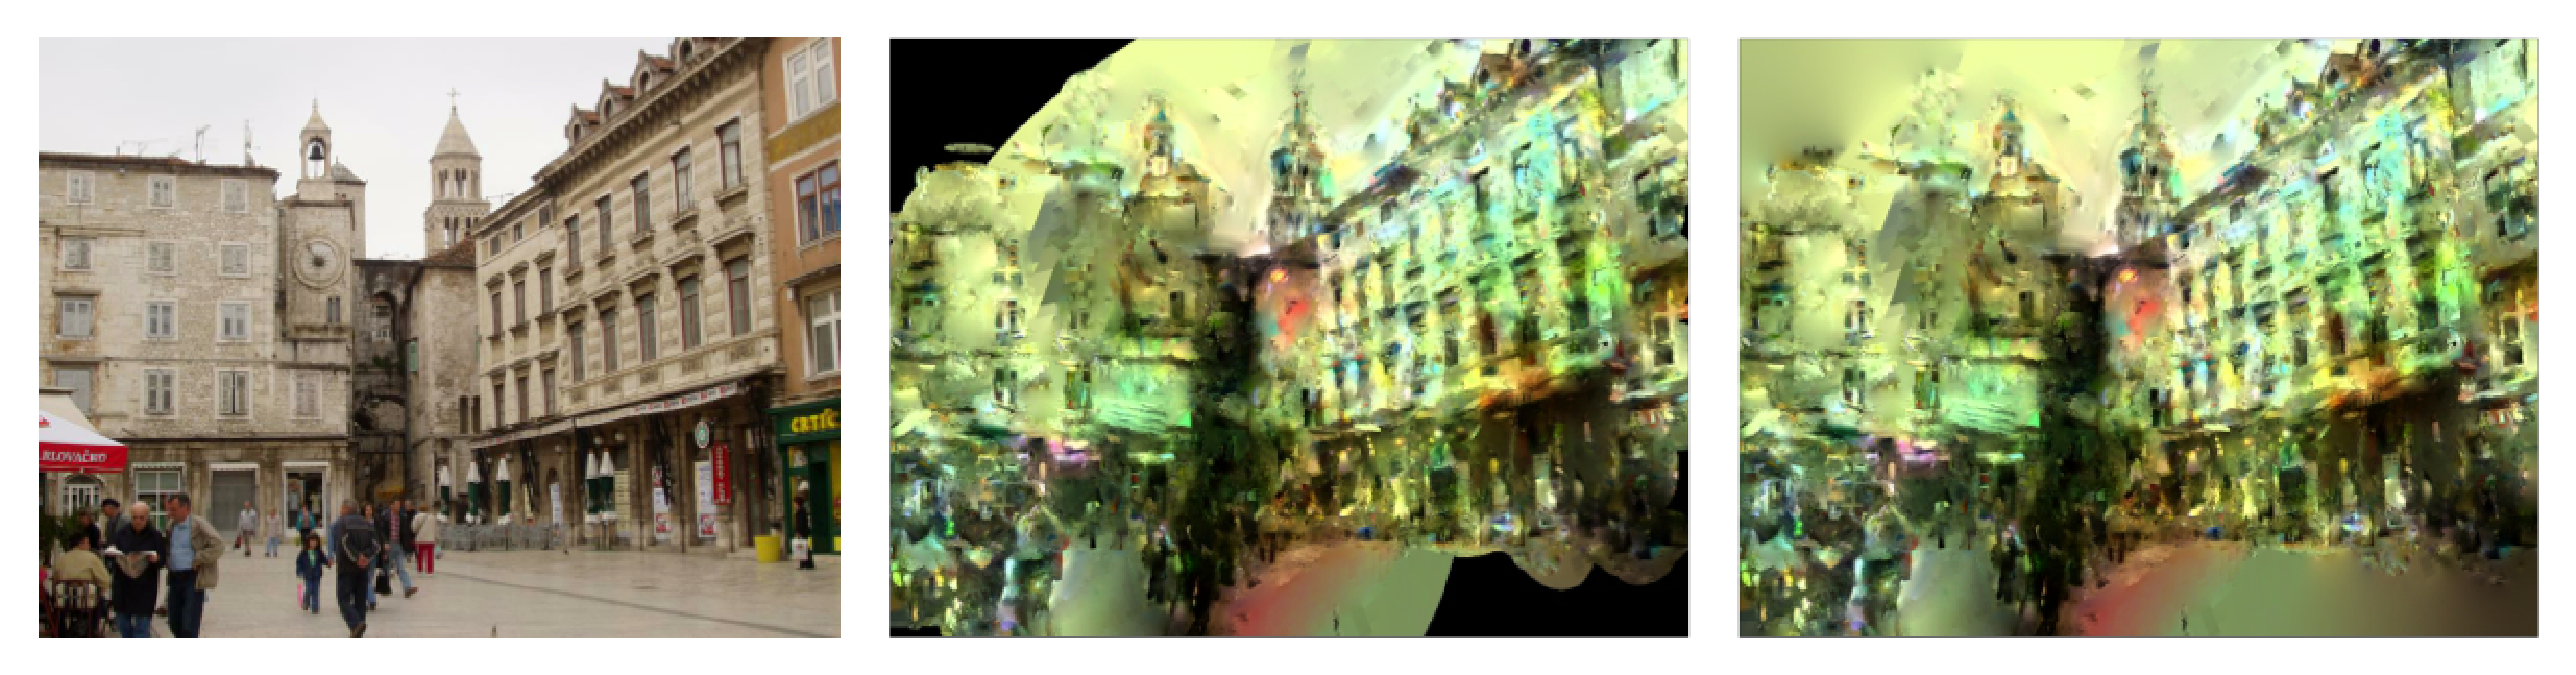
\includegraphics[width=12cm]{imgs/ch1/Weinzaepfel_res}
\caption{Weinzaepfel基于局部特征的图像重建结果,从左向右依次是原始图像、重建图像、补全后的图像}
\label{fig:Weinzaepfel_res}
\end{figure}



\section{国内外研究现状}

本文所探讨的基于局部特征的图像重建算法的脱胎于图像拼接技术和相似图像搜索技术,这两个技术相对而言较为成熟:图像拼接领域,SIFT特征的强可区分性和不变性使之广泛应用在全景图拼接领域\cite{Brown:2006ir};相似图像搜索在近年来发展较快,在搜索效率和搜索准确度两个层面进行探索,利用局部特征取代全局特征\cite{Xu:2013wc,POLICY:2013te,Wu:2009bl}以及利用局部特征的空间编码\cite{Zhou:2010tv}进行更为精确的相似图像搜索,使用min-hash等技术对特征进行压缩\cite{Chum:2008jo}提高搜索的速度。

在其上发展而来的基于局部特征的图像重建算法是近几年刚刚提出的一项新颖的技术手段,Philippe Weinzaepfel等人于2011年首先提出了基于局部特征进行图像的重建\cite{Weinzaepfel:2011jh},重建方法首先是根据局部特征使用传统技术在大数据集上找到与原始图像视觉相似的图像块,通过特征匹配与配准将候选图像块转换到标准图像域,通过无缝拼接技术将其拼合在一起,最后使用平滑差值计算空白区域的像素值,以椭圆形图像块为基本单元,重建的结果如图\ref{fig:Weinzaepfel_res}所示,在这一全自动干的图像重建系统中,虽然重建结果没有达到视觉满意程度,但是显示了基于特征进行重建的可能性,作者由此提出了图像的局部特征信息可能泄露用户隐私这一话题。

随后,Maryam Daneshi和Jiaqi Guo\cite{Daneshi:2011wi}则在确实特征尺度信息的前提下,挖掘图像重建的最大可能。他们采用方形图像块作为重建的基本单元,利用贪婪算法逐步的学习每一个图像块的尺度,完成图像的亮度信息重建,最后采用用户指定颜色遮罩并用最优化算法来进行上色,重建结果如图\ref{fig:Daneshi_res}所示,重建结果保留了大部分的图像信息。

Lican Dai等人提出将其应用在手机地标图像的实时分享\cite{Dai:2012vn},采用基于搜索的重建技术搭建了IMShare系统,提出使用缩略图来指导服务器端的特征提取和图像融合,实验结果显示缩略图的使用大大提升了图像的重建结果,该系统不仅能够重建人眼视觉满意的图像,而且采用并行的处理手段,能在秒这一数量级上完成重建流程。Huanjing Yue使用相似的技术手段进行超分辨率的图像生成,使用低分辨率(LR)的图像在大数据集上进行搜索,得到高分辨率(HR)的候选图像,再通过特征提配与图像重建的技术手段生成超分辨率图像(SR)。

\section{论文的主要研究内容与章节安排}
\subsection{主要研究内容}

本课题以文献\cite{Yue:2013gl}提出的核心任务与技术框架为基础,重点研究在基于云的图像压缩应用场景下的基于局部特征的图像重建算法,进一步探索利用更丰富的图像特征信息在大语料集中进行高质量的图像重建,使重建图像质量达到人眼主观效果较好的程度。

\subsection{章节安排}

%% 本章参考文献
\ifx\usechapbib\empty
\nocite{BSTcontrol}
\bibliographystyle{buptgraduatethesis}
\bibliography{bare_thesis}
\fi
